\documentclass{article}%
\usepackage[T1]{fontenc}%
\usepackage[utf8]{inputenc}%
\usepackage{lmodern}%
\usepackage{textcomp}%
\usepackage{lastpage}%
\usepackage{authblk}%
\usepackage{graphicx}%
%
\title{Invasiveness and anchorage independent growth ability augmented by PTEN inactivation through the PI3K/AKT/NFkB pathway in lung cancer cells}%
\author{Edward Cooper}%
\affil{Department of Surgery, Faculty of Medicine, School of Medicine, Kaohsiung Medical University, Kaohsiung, Taiwan}%
\date{01{-}01{-}2014}%
%
\begin{document}%
\normalsize%
\maketitle%
\section{Abstract}%
\label{sec:Abstract}%
What you should think about when you turn on your blue light.\newline%
Its the same blue light that looks like a toxic cloud floating over your body.\newline%
Previous research has linked dark blue light with atherosclerosis, atherosclerosis, heart attacks and strokes.\newline%
So now researchers are looking for a new way to dim the blue light and give you a red light.\newline%
A team of researchers from UCLA got Dr. Cari Ben{-}Khabib to figure out just how dark the blue light is and turn it off.\newline%
She led the study.\newline%
It worked, until about 10 seconds in it was completely off.\newline%
Then they switched the blue light back on.\newline%
We were up to about 17 minutes before {[}the blue light{]} went off, and it seems like it went about 12 minutes before it went off. Thats normal, Ben{-}Khabib said.\newline%
The same researchers also tested the sleep patterns of 25 people and found that those that couldnt sleep on the blue light werent as alert as people who could fall asleep on normal

%
\subsection{Image Analysis}%
\label{subsec:ImageAnalysis}%


\begin{figure}[h!]%
\centering%
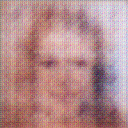
\includegraphics[width=150px]{500_fake_images/samples_5_38.png}%
\caption{A Man With A Beard And A Beard Wearing A Tie}%
\end{figure}

%
\end{document}